{\Large {Preliminary Analysis}}
\\
The CBECS survey results are available in csv format on the EIA website, labeled as a microdata file. \footnote{\href{https://www.eia.gov/consumption/commercial/data/2012/index.php?view=microdata}{microdata - \url{https://www.eia.gov/consumption/commercial/data/2012/index.php?view=microdata}}}  This file consists of 6,720 records that represent an estimated 5.6 million total buildings in the United States, using a complex sampling design that is explained in the accompanied user's guide.  This data set consists of 1,119 variables, which include various major fuel consumption values, such as electricity, natural gas, etc.  From initial inspection on these proposed response variables, after normalizing per square foot, it appears that they have a unimodal right skew.  All fuel sources appear to be operating on relatively the same scale with a few high usage cases that may or may not be outliers. \\

\begin{figure}[h]
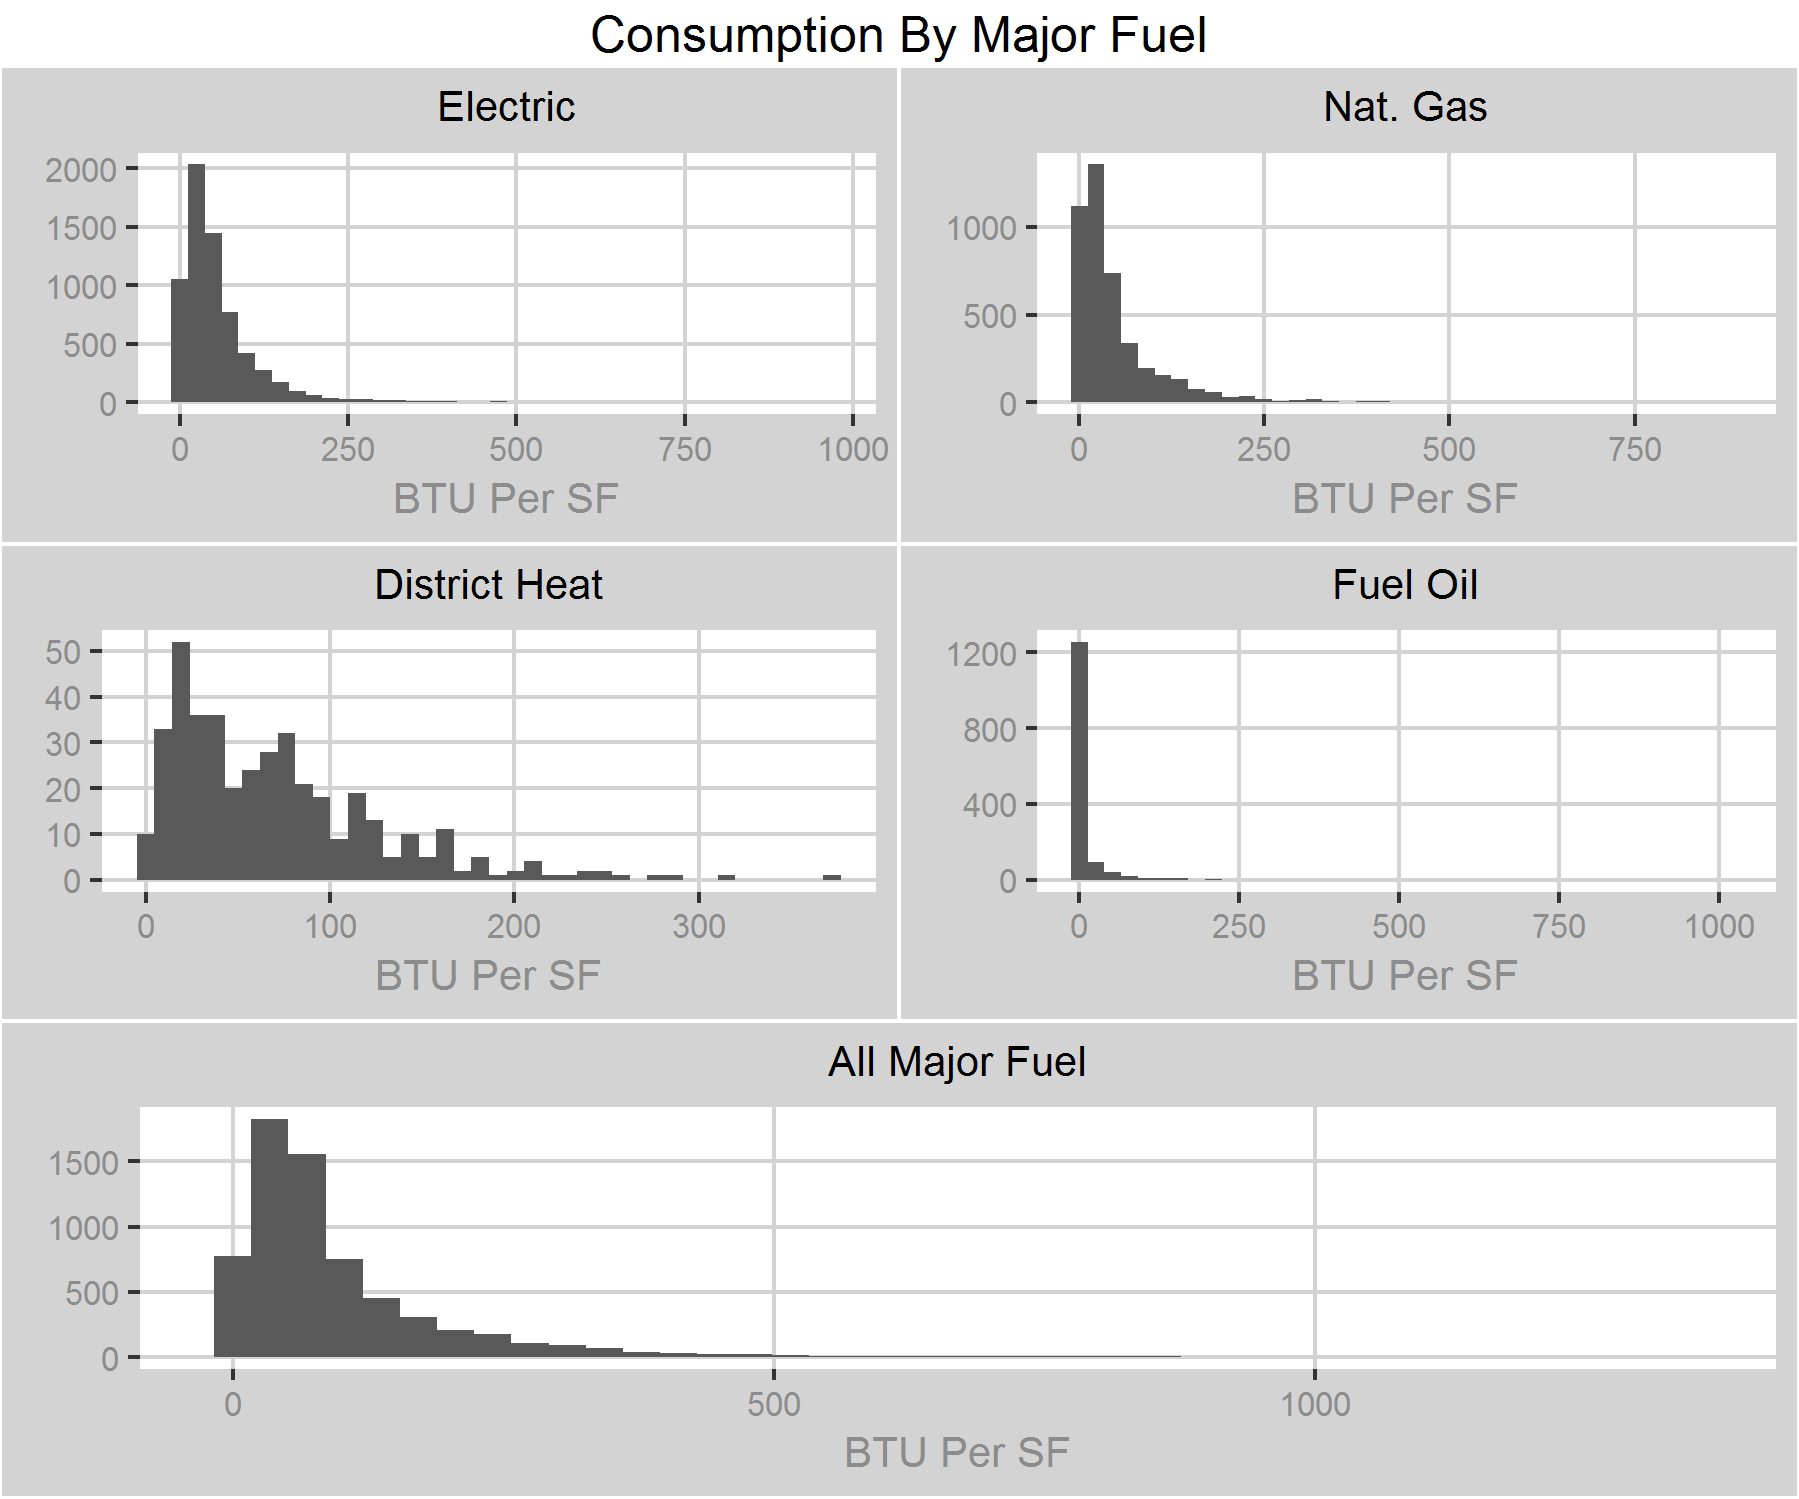
\includegraphics[width=\textwidth]{major_fuels_preliminary_analysis.png}
\centering
\end{figure}
